\chapter[PAC-Bayesian Theory for the Robust Majority Vote]{PAC-Bayesian Theory for\\ the Robust Majority Vote}
\label{chap:mv-robustness}
\addchapterlof
\addchapterloe
\addchapterloa

\vspace{-1.0cm}
\begin{center}
\textbf{This chapter is based on the following paper}\\[0.1cm]
\end{center}
\printpublication{ViallardVidotHabrardMorvant2021}

\vspace{0.3cm}

\minitoc

\begin{abstract}
In this chapter, we derive the first general PAC-Bayesian generalization bounds for adversarial robustness, that estimate, how much the majority vote will be robust to imperceptible perturbations in the input.
Instead of deriving a worst-case analysis of the risk of the majority vote over all the possible perturbations, we leverage the PAC-Bayesian framework recalled in \Cref{chap:pac-bayes} to bound the averaged risk on the perturbations.
Our theoretically founded analysis has the advantage to provide general bounds {\it (i)} that are valid for any kind of adversarial attacks, {\it (ii)} that are tight, {\it (iii)} that can be directly minimized in a self-bounding algorithm to obtain a robust majority vote.
We empirically show this robustness on different attacks.
\end{abstract}

\newpage

\section{Introduction}

In this chapter, we first formalize in \Cref{chap:mv-robustness:section:adversarial-robust-pac-bayes} the notion of majority vote for the adversarial robustness setting. 
To do so, we adapt the majority vote (recalled in \Cref{chap:pac-bayes} for supervised learning) by assuming that the inputs can be slightly modified/perturbed to fool the prediction of the majority vote, often in a malicious way; this setting is called {\it adversarial robustness}.
The existence of such modified inputs, known as {\it adversarial examples}~\citep{BiggioCoronaMaiorcaNelsonSrndicLaskovGiacintoRoli2013,SzegedyZarembaSutskeverBrunaErhanGoodfellowFergus2014} and illustrated in \Cref{chap:mv-robustness:fig:examples}.

\begin{figure}[H]
    \centering
    \includestandalone[width=1.0\textwidth]{chapter_3/figures/introduction}
    \caption[Illustration of the Adversarial Examples]{
    On the left, the original image is predicted correctly by the classifier as ``cat''. 
    The middle image corresponds to a perturbation/noise added to this original image.
    On the right, by applying the perturbation on the original image, the result is an image that looks identical to the original to the human eye, however, the prediction changes radically.
    This result image with the imperceptible perturbation is called an adversarial example.}
    \label{chap:mv-robustness:fig:examples}
\end{figure}

The models (\ie, the majority vote in our case) must be robust to these small inputs' perturbations to better guarantees the user safety.
Indeed, when machine learning models are applied to real problems, such as autonomous vehicles, the perturbations must not compromise the safety of the users.
The perturbed examples is obtained from an {\it adversarial attack} that fools the considered model while the {\it adversarial defense} techniques enhance the adversarial robustness to make the attacks useless \citep[see \eg,][]{PapernotMcDanielJhaFredriksonBerkayCelikSwami2016,GoodfellowShlensSzegedy2015,MadryMakelovSchmidtTsiprasVladu2018,CarliniWagner2017, ZantedeschiNicolaeRawat2017, KurakinGoodfellowBengio2017}.
However, the majority votes and many other models lack guarantees on the robustness.
To tackle this issue, we propose to formulate the adversarial robustness through the lens of the PAC-Bayesian theory recalled in \Cref{chap:pac-bayes}; we call here our setting the {\it adversarially robust PAC-Bayes}.\\

The idea consists in considering an {\it averaged adversarial robustness risk} corresponding to the probability that the model misclassifies a perturbed example (this can be interpreted as an averaged risk over the perturbations). 
We also define an {\it averaged-max adversarial risk} as the probability that there exists at least one perturbation that leads to a misclassification.
These definitions, based on averaged quantities, have the advantage {\it (i)} of being suitable for the PAC-Bayesian framework and majority vote classifiers, and {\it (ii)} of being related to the classical adversarial robustness risk.
Then, for each of our adversarial risks, we derive a PAC-Bayesian generalization bound that is valid to any kind of attack.
From an algorithmic point of view, these bounds are directly minimizable to learn a majority vote robust in average to attacks.
Since we directly minimize a generalization bound, our algorithms stand in the class of {\it self-bounding algorithms}~\citep{Freund1998}.
We empirically illustrate that our framework is able to provide generalization guarantees with non-vacuous bounds for the adversarial risk while ensuring efficient protection to adversarial attacks.\\ 

Note that all the proofs of this chapter are deferred in \Cref{ap:mv-robustness}.


\section{Adversarially Robust Majority Vote}
\label{chap:mv-robustness:section:adversarial-robust-pac-bayes}

\subsection{Setting}

We mainly adopt the setting of \Cref{chap:pac-bayes}.
We tackle {\it binary} classification tasks with the input space $\X{=}\R^\d$ and the output/label space $\Y=\{-1,+1\}$.
We assume that $\D$ is a fixed but unknown distribution on $\X{\times}\Y$.
An example is denoted by $(\x,\y) \in\X{\times}\Y$.
Let $\S\!=\!\{(\x_i,\y_i)\}_{i=1}^{\m}$ be the learning sample of $\m$ examples {\it i.i.d.} sampled from $\D$; 
We denote the distribution of such $\m$-sample by $\D^\m$.
Let $\H$ be a set of real-valued voters from $\X$ to $[-1, +1]$.
Assuming the voters set $\H$ and a learning sample $\S$, our goal is to learn a well-performing $\Q$-weighted majority vote defined in \Cref{chap:pac-bayes:majority-vote} by
\begin{align*}
\forall \x\in\X,\quad \MVQ(\x) = \sign\LB \EE_{\h\sim \Q} \h(\x) \RB.
\end{align*}

One wants to find a $\Q$-weighted majority vote that minimizes the true risk $\Risk_{\D}(\MVQ)$ on $\D$ defined in \Cref{chap:pac-bayes:def:mv-risk} as
\begin{align*}
\Risk_{\D}(\MVQ) \triangleq \EE_{(\x, \y)\sim\D} \indic\LB \MVQ(\x) \ne \y\RB.
\end{align*}

\looseness=-1
However, in real-life applications, an imperceptible perturbation of the input can have a bad influence on the classification performance on unseen data \citep{SzegedyZarembaSutskeverBrunaErhanGoodfellowFergus2014}: the usual generalization guarantees do not stand anymore.
Such an imperceptible perturbation can be modeled by a (relatively small) additive noise $\epsilon$ applied an input $\x$ leading to a perturbed input $\x+\epsilon$.
Let $b\!>\!0$ and $\LM\cdot\RM$ be an arbitrary norm, the set of possible noises $\Xpert$ is defined by\footnote{The most used norms in the set of possible noises are the $\ell_1$, $\ell_2$ and $\ell_\infty$-norms.}
\begin{align*}
\Xpert{=}\big\{ \epsilon\in\R^\d  \,\big|\, \LM \epsilon\RM \le b\big\}.
\end{align*}

The learner aims now to find an {\it adversarial robust} classifier that is robust in average to all noises in $\Xpert$ over $(\x,\y)\sim\D$.
More formally, one wants to minimize the true adversarial risk $\RiskA_{\D}(\MVQ)$ defined in the following definition.

\begin{definition}[True/Empirical Adversarial Risk] For any distribution $\D$ on $\X\times\Y$, for any distribution $\Q$ on $\H$, the {\it true adversarial risk} is defined as
\begin{align*}
    \RiskA_{\D}(\MVQ) = \EE_{(\x,\y)\sim\D}\max_{\epsilon\in\Xpert}\ 
    \indic\LB\MVQ(\x{+}\epsilon)\ne \y\RB.
\end{align*}
Since $\D$ is unknown, $\RiskA_{\D}(\MVQ)$ cannot be directly computed, then one usually deals with the empirical adversarial risk defined as
\begin{align*}
\RiskA_{\dS}(\MVQ) = \frac{1}{\m}\sum_{i=1}^{\m}\max_{\epsilon\in\Xpert}\ \indic\LB\MVQ(\x_i{+}\epsilon)\ne \y_i\RB.
\end{align*}
\label{chap:mv-robustness:def:rob-risk}
\end{definition}

In this chapter, our objective is to try to make the majority vote classifier $\MVQ$ robust to {\it adversarial attacks} that aim at finding an {\it adversarial example} $\x+\epsilon^*(\x{,}\y)$ to fool $\MVQ()$ for given example $(\x,\y)$, where $\epsilon^*(\x{,}\y)$ is defined as
\begin{align}
    \epsilon^*(\x{,}\y) \,\in\, \argmax_{\epsilon\in\Xpert}\ \indic\LB\MVQ(\x{+}\epsilon)\ne \y\RB.\label{chap:mv-robustness:eq:adv-max}
\end{align}
In consequence, {\it adversarial defense} mechanisms often rely on the adversarial attacks by replacing the original examples $(\x,\y)$ with the adversarial ones $(\x+\epsilon^*(\x,\y),\y)$ during the learning phase; this procedure is called adversarial training.
Even if there are other defenses, as we will see later, adversarial training appears to be one of the most efficient defense mechanisms~\citep{RenZhengQinLiu2020}.
Optimizing \Cref{chap:mv-robustness:eq:adv-max} is however intractable due to the non-convexity of $\MVQ$ induced by the \text{sign} function.
The adversarial attacks of the existing frameworks in the literature (that we discuss in \Cref{chap:mv-robustness:related-works}) aim at finding the optimal perturbation $\epsilon^*(\x{,}\y)$, but, in practice, one considers an approximation of this perturbation.

\subsection{Related Works}
\label{chap:mv-robustness:related-works}

\paragraph{Adversarial Attacks/Defenses.} 
Numerous methods\footnote{The reader can refer to \citet{RenZhengQinLiu2020} for a survey on adversarial attacks and defenses.} exist to solve--- or approximate ---the optimization of \Cref{chap:mv-robustness:eq:adv-max}.
Among them, the Fast Gradient Sign Method (\FGSM) of~\citet{GoodfellowShlensSzegedy2015} is an attack consisting in generating a noise $\epsilon$ in the direction of the gradient of the loss function with respect to the \mbox{input $\x$}.
\citet{KurakinGoodfellowBengio2017}  introduced \IFGSM, an iterative version of \FGSM: at each iteration, one repeats \FGSM and adds to $\x$ a noise, that is the sign of the gradient of the loss with respect to $\x$.
Following the same principle as \IFGSM, \citet{MadryMakelovSchmidtTsiprasVladu2018} proposed a method based on Projected Gradient Descent (\PGD) that includes a random initialization of $\x$ before the optimization.
Another technique known as the {\it Carlini and Wagner Attack}~\citep{CarliniWagner2017} aims at finding adversarial examples $\x+\epsilon^*(\x{,}\y)$ that are as close as possible to the original $\x$, \ie, they want an attack being the most imperceptible as possible. 
However, producing such imperceptible perturbation leads to a high-running time in practice.
Contrary to the most popular techniques that look for a model with a low adversarial robust risk, our work stands in another line of research where the idea is to relax this  worst-case risk measure by considering an {\it averaged} adversarial robust risk over the noises instead of a  $\max$-based formulation \citep[see, \eg,][]{ZantedeschiNicolaeRawat2017,HendrycksDietterich2019}. 
Our averaged formulation is introduced in the \Cref{chap:mv-robustness:section:adversarial-robust-pac-bayes}.

\paragraph{Generalization Bounds for Adversarial Robustness.}
Recently, few generalization bounds for adversarial robustness have been introduced \citep[\eg,][]{KhimLoh2018,YinRamchandranBartlett2019,MontasserHannekeSrebro2019,MontasserHannekeSrebro2020,CohenRosenfeldZicoKolter2019,SalmanLiRazenshteynZhangZhangBubeckYang2019,PinotMeunierAraujoKashimaYgerGouyPaillerAtif2019,PinotMeunierYgerGouyPaillerChevaleyreAtif2022}.
\citeauthor{KhimLoh2018}, and \citeauthor{YinRamchandranBartlett2019}'s results are Rademacher complexity-based bounds. 
The former makes use of a surrogate of the adversarial risk; the latter provides bounds in the specific case of neural networks and linear classifiers and involves an unavoidable polynomial dependence on the dimension of the input.
\citeauthor{MontasserHannekeSrebro2020}
study robust PAC-learning for PAC-learnable classes with finite VC-dimension for unweighted majority votes that have been ``robustified'' with a boosting algorithm. 
However, their algorithm requires to consider all possible adversarial perturbations for each example, which is intractable in practice, and their bound also suffers from a large constant as indicated at the end of the \citet[Theorem 3.1][]{MontasserHannekeSrebro2019}'s proof.
\citeauthor{CohenRosenfeldZicoKolter2019} provide bounds that estimate what is the minimum noise to get an adversarial example (in the case of perturbations expressed as Gaussian noise) while our results give the probability of being fooled by an adversarial example.
\citeauthor{SalmanLiRazenshteynZhangZhangBubeckYang2019} leverage \citeauthor{CohenRosenfeldZicoKolter2019}'s method and adversarial training in order to get tighter bounds.
Moreover, \citeauthor{FarniaZhangTse2019} present margin-based bounds on the adversarial robust  risk for specific neural networks and attacks (such as \FGSM or \PGD).
While they made use of a classical PAC-Bayes bound, their result is not a PAC-Bayesian analysis  and stands in the family of uniform-convergence bounds \citep[see][Ap.~J for details]{NagarajanKolter2019}. 
In this thesis, we provide PAC-Bayesian bounds for general models expressed as majority votes, their bounds are thus not directly comparable to ours.

\subsection{PAC-Bayesian Adversarial Risks}

Instead of looking for the noise from \Cref{chap:mv-robustness:eq:adv-max} that maximizes the chance of fooling the algorithm, we propose to model the perturbation according to an example-dependent distribution.
This example-dependent distribution is further used to define our new risks.
First let us define $\DX$ a distribution, on the set of possible noises 
$\Xpert$, that is dependent on an example $(\x,\y)\in\X{\times}\Y$. 
Then, we denote as $\Dpert$ the distribution on $(\X{\times}\Y){\times}\Xpert$ defined as
\begin{align*}
\Dpert((\x,\y), \epsilon) = \D(\x,\y)\cdot\DX(\epsilon),
\end{align*}
which further permits to generate \textit{perturbed examples}.
For a given example $(\x_i,\y_i){\sim}\D$, we consider a set of $n$ perturbations sampled from $\DXi$ denoted by $\Epert_i{=}\{\epsilon^i_{j}\}_{j=1}^{n}$.
Then we consider as a learning set the \mbox{$m{\times} n$-sample} $\Spert=\LC ( (\x_i,\y_i), \Epert_i)\RC_{i=1}^\m \in (\X{\times}\Y{\times}\Xpert^n)^{\m}$.
In other words, each $( (\x_i,\y_i), \Epert_i)\in\Spert$ is sampled from a distribution that we denote by $\Dpert^{n\!}$ such that
\begin{align*}
\Dpert^{n}((\x_i,\y_i), \Epert_i)=\D(\x_i,\y_i){\cdot}\prod_{j=1}^{n}\DXi(\epsilon^i_{j}).
\end{align*}

Furthermore, we denote as $(\Dpert^n)^\m$ the empirical distribution on the perturbed learning sample consisted of $\m$ examples and $n$ perturbations for each example.
Then, inspired by the works of \citet{ZantedeschiNicolaeRawat2017,HendrycksDietterich2019}, we define our {\it robustness averaged adversarial risk} as follows.
\begin{definition}[Averaged Adversarial Risk]
\label{chap:mv-robustness:def:average_rob_risk}
For any distribution $\Dpert$ on $(\X{\times}\Y){\times}\Xpert$, for any distribution $\Q$ on $\H$, the averaged adversarial risk of $\MVQ$ is defined as
\begin{align*}
\Risk_{\Dpert}(\MVQ) \ &=\  \PP_{((\x,\y), \epsilon)\sim \Dpert}(\MVQ(\x+\epsilon) \neq \y)\ \\
&=\ \EE_{((\x,\y), \epsilon)\sim \Dpert}\indic\LB\MVQ(\x+\epsilon) \neq \y\RB.
\end{align*}
The empirical averaged adversarial risk is computed on a $m{\times}n$-sample $\Spert=\LC \LP (\x_i,\y_i), \Epert_i\RP\RC_{i=1}^{\m}$ is 
\begin{align}
 \nonumber\Risk_{\dSpert}(\MVQ) &= 
    \frac{1}{mn} \sum_{i=1}^\m\sum_{j=1}^n \indic\LB\MVQ(\x_i+\epsilon^i_j) \neq \y_i\RB.
\end{align}
\end{definition}
As we will show in \Cref{chap:mv-robustness:proposition:risks},  the risk $\Risk_{\Dpert}(\MVQ)$ is considered optimistic regarding $\epsilon^*(\x{,}\y)$ of \Cref{chap:mv-robustness:eq:adv-max}.
Indeed, instead of taking the $\epsilon$ maximizing the loss, the $\epsilon$ is drawn from a distribution.
Hence, it can lead to a non-informative risk if the $\epsilon$ are not informative enough to fool the classifier.
To overcome this, we propose an extension that we refer as 
{\it averaged-max \mbox{adversarial risk}}. 
Note that we abuse the notation of the adversarial true risk defined in \Cref{chap:mv-robustness:def:rob-risk}.

\begin{definition}[Averaged-Max Adversarial Risk]
\label{chap:mv-robustness:def:average_max_risk}
 For any distribution $\Dpert$ on $(\X{\times}\Y){\times}\Xpert$, for any distribution $\Q$ on $\H$, the averaged-max adversarial risk of $\MVQ$ is defined as
\begin{align*}
\RiskM_{\Dpert^{n\!}}(\MVQ) = \PP_{((\x,\y), \Epert)\sim\Dpert^{n\!}} \big( \exists\, \epsilon\in\Epert, \MVQ(\x+\epsilon) \ne \y \big). 
\end{align*}
The empirical averaged-max adversarial risk  computed on a $m\!\times\!n$-sample $\Spert=\{( (\x_i,\y_i), \Epert_i )\}_{i=1}^{\m}$ is
\begin{align*}
\RiskM_{\dSpert}(\MVQ) &= \frac{1}{\m} \sum_{i=1}^\m \max_{\epsilon\in\Epert_i}\indic\LB\MVQ(\x_i+\epsilon) \neq \y_i\RB.
\end{align*}
\end{definition}
For an example $(\x,\y){\sim}\D$, instead of checking if one perturbed example $\x{+}\epsilon$ is  adversarial, we sample $n$ perturbed examples $\x{+}\epsilon_1,\ldots, \x{+}\epsilon_n$ and we check if at least one example is adversarial.

\section{Adversarially Robust PAC-Bayes}

We show in \Cref{chap:mv-robustness:sec:relation} the relations between the different risks.
\Cref{chap:mv-robustness:sec:bound} introduces the PAC-Bayesian bounds to assess the robustness of the majority vote.

\subsection{Relations Between the Adversarial Risks} 
\label{chap:mv-robustness:sec:relation}
\Cref{chap:mv-robustness:proposition:risks} below shows the intrinsic relationships between the classical adversarial risk $\RiskA_{\D}(\MVQ)$ and our two relaxations $\Risk_{\Dpert}(\MVQ)$ and $\RiskM_{\Dpert^{n\!}}(\MVQ)$.
In particular, \Cref{chap:mv-robustness:proposition:risks} shows that the larger number of perturbed examples $n$, the higher is the chance to get an adversarial example and then to be close to the adversarial risk $\RiskA_{\D}(\MVQ)$.

\begin{restatable}[Relations Between the Averaged Adversarial Risks]{proposition}{proprisks}\label{chap:mv-robustness:proposition:risks} 
For any distribution $\Dpert$ on $(\X{\times}\Y){\times}\Xpert$, for any distribution $\Q$ on $\H$, for any \mbox{$(n, n')\in\mathbb{N}^2$}, with \mbox{$1 \le {n'} \le {n}$}, we have
\begin{align}
    \Risk_{\Dpert}(\MVQ)\ \le\ \RiskM_{\Dpert^{{n'}}}(\MVQ)\ \le\ \RiskM_{\Dpert^{{n}}}(\MVQ)\ \le\  \RiskA_{\D}(\MVQ).\label{chap:mv-robustness:eq:risks_inequalities}
\end{align}
\end{restatable}
\begin{noaddcontents}\begin{proof}
Deferred to~\Cref{ap:mv-robustness:sec:proof-risks}.
\end{proof}\end{noaddcontents}

The left-hand side of \Cref{chap:mv-robustness:eq:risks_inequalities} confirms that the averaged adversarial risk $\Risk_{\Dpert}(\MVQ)$ is optimistic regarding the classical  $\RiskA_{\D}(\MVQ)$.
\Cref{chap:mv-robustness:proposition:avg-worst-risk} estimates how close  $\Risk_{\Dpert}(\MVQ)$ can be to $\RiskA_{\D}(\MVQ)$.

\begin{restatable}[Classical and Averaged Adversarial Risks]{proposition}{propavgworstrisk}\label{chap:mv-robustness:proposition:avg-worst-risk}
For any  distribution $\Dpert$ on $(\X\times\Y)\times\Xpert$, for any distribution $\Q$ on $\H$, we have
\begin{align*}
    &\RiskA_{\D}(\MVQ) - \TV(\gamma\|\Gamma)\ \le\  \Risk_{\Dpert}(\MVQ),
\end{align*}
where $\Gamma$ and $\gamma$ are distributions on $\X{\times}\Y$ and $\TV(\gamma\|\Gamma) = \EE_{(\x', \y')\sim\Gamma}\frac{1}{2}\LN\frac{\gamma(\x'{,}\y')}{\Gamma(\x'{,}\y')}{-}1\RN,$
is the Total Variation (TV) distance between $\gamma$ and $\Gamma$.\\
The density $\Gamma(\x',\y')$ corresponds to the probability of drawing a perturbed example $(\x', \y')= (\x{+}\epsilon, \y)$ with ${((\x,\y),\epsilon){\sim}\Dpert}$, \ie, we have
\begin{align*}
\Gamma(\x', \y') = \!\!\Pr_{((\x,\y),\epsilon){\sim}\Dpert}\LB \x{+}\epsilon=\x',\  \y=\y'\RB.
\end{align*}
The density $\gamma(\x',\y')$ is the probability to draw an adversarial example $(\x', \y')=(\x{+}\epsilon^*(\x{,}\y),\y)$ with $(\x,\y){\sim}\D$, \ie, we have
\begin{align*}
\gamma(\x', \y') =\!\! \Pr_{(\x,\y)\sim\D}\LB \x{+}\epsilon^*(\x,\y)=\x',\  \y=\y'\RB.
\end{align*}
\end{restatable}
\begin{noaddcontents}\begin{proof}
Deferred to~\Cref{ap:mv-robustness:sec:proof-avg-worst-risk}.
\end{proof}\end{noaddcontents}

Note that $\epsilon^*(\x{,}\y)$ depends on $\Q$, hence $\gamma$ depends on $\Q$.
From \Cref{chap:mv-robustness:proposition:avg-worst-risk} and the distributions $\Gamma$ and $\gamma$, the risks 
$\RiskA_{\D}(\MVQ)$  and $\Risk_{\Dpert}(\MVQ)$ can be rewritten as
\begin{align*}
    &\Risk_{\Dpert}(\MVQ) = \Pr_{(\x', \y')\sim\Gamma}\LB \MVQ(\x')\ne \y'\RB,\\
    \text{and}\quad &\RiskA_{\D}(\MVQ) = \Pr_{(\x',\y'){\sim}\gamma}\LB \MVQ(\x')\ne \y'\RB.
\end{align*}
Finally, Propositions~\ref{chap:mv-robustness:proposition:risks} and~\ref{chap:mv-robustness:proposition:avg-worst-risk} relate the adversarial risk $\Risk_{\Dpert}(\MVQ)$ to the ``standard'' adversarial risk $\RiskA_{\D}(\MVQ)$.
Indeed, from the two propositions we obtain
\begin{align}
\label{chap:mv-robustness:eq:merged_prop}
    \RiskA_{\D}(\MVQ) - \TV(\gamma\|\Gamma)\ \le\  \Risk_{\Dpert}(\MVQ)\ \le\  \RiskM_{\Dpert^{n\!}}(\MVQ)\ \le\  \RiskA_{\D}(\MVQ).
\end{align}
Hence, the smaller the TV distance $\TV(\gamma\|\Gamma)$, the closer the averaged adversarial risk $\Risk_{\Dpert}(\MVQ)$ is from $\RiskA_{\D}(\MVQ)$ and the more probable an example $((\x,\y),\epsilon)$ sampled from $\Dpert$ would be adversarial, \ie,
when our ``averaged'' adversarial example looks like a ``specific'' adversarial example.
Moreover, \Cref{chap:mv-robustness:eq:merged_prop} justifies that the PAC-Bayesian point of view makes sense for adversarial learning with theoretical guarantees: the PAC-Bayesian guarantees we derive in the next section for our adversarial risks implies guarantees on the adversarial risk $\RiskA_{\D}(\MVQ)$.

\subsection{PAC-Bayesian Bounds on the Adversarially Robust Majority Vote}
\label{chap:mv-robustness:sec:bound}

To derive PAC-Bayesian generalization bounds on the risk $\Risk_{\Dpert}(\MVQ)$, respectively on $\RiskM_{\Dpert^{n\!}}(\MVQ)$, we consider one of the classical surrogates, \ie, the Gibbs risk~(\Cref{chap:pac-bayes:def:gibbs}), defined below in \Cref{chap:pac-bayes:eq:gibbs}, respectively \Cref{chap:pac-bayes:eq:gibbs-max}.

\begin{definition}[Surrogates on the Averaged Adversarial Risks] For any distribution $\Dpert$ on $(\X{\times}\Y)\times\Epert$, for any hypothesis set $\H$, for any $\Q$ on $\H$,  
\begin{align}
  \RiskS_{\Dpert}(\Q) &= \EE_{((\x,\y),\epsilon)\sim\Dpert} \frac{1}{2}\left[ 1 {-}  \EE_{\h\sim\Q} \y\h(\x{+}\epsilon) \right],\label{chap:pac-bayes:eq:gibbs}\\ 
    \text{and}\quad
    \RiskMS_{\Dpert^{n}}(\Q) &= \EE_{((\x,\y),\Epert)\sim\Dpert^{n}} \frac{1}{2}\left[ 1{-}\min_{\epsilon\in\Epert} \Big( \y\! \EE_{\h\sim\Q} \h(\x{+}\epsilon)\Big)\right].\label{chap:pac-bayes:eq:gibbs-max}
\end{align}
\end{definition}

Put into words, these surrogates are expressed as the expectation over $\Q$ of the individual risks of the voters involved in $\H$. 
From an algorithmic perspective, $\RiskS_{\Dpert}(\Q)$ and $\RiskMS_{\Dpert^{n}}(\Q)$ have the advantages {\it (i)} of being differentiable contrary to $\Risk_{\Dpert}(\MVQ)$ and $\RiskM_{\Dpert^{n\!}}(\MVQ)$, and {\it (ii)} to upper-bound to $\Risk_{\Dpert}(\MVQ)$ and $\RiskM_{\Dpert^{n\!}}(\MVQ)$ as follows.

\begin{restatable}[Upper Bounds on the Surrogates]{theorem}{theoremadvergibbs}\label{chap:mv-robustness:theorem:2-adver-gibbs}
For any distributions $\Dpert$ on $(\X{\times}\Y){\times}\Xpert$ and $\Q$ on $\H$, \mbox{for any $n\!>\!1$, we have}
\begin{align*}
    \Risk_{\Dpert}(\MVQ) \le 2  \RiskS_{\Dpert}(\Q), \qquad\text{and} \qquad \RiskM_{\Dpert^{n\!}}(\MVQ) \le 2  \RiskMS_{\Dpert^{n}}(\Q).
\end{align*}
\end{restatable}
\begin{noaddcontents}\begin{proof}
Deferred to~\Cref{ap:mv-robustness:sec:proof-2-adver-gibbs}.
\end{proof}\end{noaddcontents}

This theorem implies that a generalization bound on $\RiskS_{\Dpert}(\Q)$, resp $\RiskMS_{\Dpert^{n}}(\Q)$ leads to a generalization bound on $\Risk_{\Dpert}(\MVQ)$, \resp, $\RiskM_{\Dpert^{n\!}}(\MVQ)$.
\Cref{chap:mv-robustness:theorem:chromatic} \resp \Cref{chap:mv-robustness:theorem:bound-average-max} below presents our PAC-Bayesian generalization bounds for $\RiskS_{\Dpert}(\Q)$ \resp $\RiskMS_{\Dpert^{n}}(\Q)$.

\begin{restatable}[PAC-Bayesian Bound on $\RiskS_{\Dpert}(\Q)$]{theorem}{theoremchromatic}\label{chap:mv-robustness:theorem:chromatic} For any distribution $\Dpert$ on $(\X{\times}\Y){\times}\Xpert$, for any set of voters $\H$, for any prior $\P\in\M*(\H)$ on $\H$, for any $n\in\N_{*}$, with probability at least $1{-}\delta$ over~$\Spert\sim(\Dpert^{n\!})^\m$, for all posteriors $\Q\in\M(\H)$ on $\H$, we have
\begin{align}
    & \kl(\RiskS_{\Spert}(\Q)\|\RiskS_{\Dpert}(\Q)) \le \frac{1}{\m} \LB\KL(\Q\|\P)+\ln\frac{\m+1}{\delta} \RB, \label{chap:mv-robustness:eq:seeger-chromatic}\\
    \text{and}\quad&\RiskS_{\Dpert}(\Q) \le \RiskS_{\Spert}(\Q)+\sqrt{\frac{1}{2\m}\LB \KL(\Q\|\P)+\ln \frac{m+1}{\delta}\RB},\label{chap:mv-robustness:eq:mcallester-chromatic}\\
    \nonumber\text{where}\quad& \RiskS_{\Spert}(\Q) = \frac{1}{\m n}\sum_{i=1}^{\m}\sum_{j=1}^n\frac{1}{2}\LB 1{-} \y_i\!\EE_{\h\sim\Q}\h(\x_i{+}\epsilon^i_j) \RB.
\end{align}
\end{restatable}
\begin{noaddcontents}\begin{proof}
Deferred to~\Cref{ap:mv-robustness:sec:proof-chromatic}.
\end{proof}\end{noaddcontents}

It is important to mention that the empirical counterpart of $\RiskS_{\Dpert}(\Q)$ is computed on $\Spert$ which is composed of non identically independently distributed samples, meaning that a ``classical'' proof technique is not applicable.
The trick here is to make use of a result of \citet{RalaivolaSzafranskiStempfel2010} that provides a {\it chromatic PAC-Bayesian bound}, \ie, a bound which supports non-independent data. 
Surprisingly, this theorem states bounds that do not depend on the number of perturbed examples $n$ but only on the number of original examples $\m$.
The reason is that the $n$ perturbed examples are  inter-dependent (see the proof in Appendix).
Note that \Cref{chap:mv-robustness:eq:seeger-chromatic} is expressed as a \citet{Seeger2002}'s bound and is tighter but less interpretable than \Cref{chap:mv-robustness:eq:mcallester-chromatic} expressed as a~\citet{McAllester1998}'s bound; these bounds involve the usual trade-off between the empirical risk $\RiskS_{\Spert}(\Q)$ and $\KL(\Q\|\P)$.

We now state a generalization bound for $\RiskMS_{\Dpert^{n}}(\Q)$.
Since this value involves a minimum term, we cannot use the same trick as for \Cref{chap:mv-robustness:theorem:chromatic}. 
To bypass this issue, we use the TV distance between two ``artificial'' distributions on $\Epert_i$.
Given $((\x_i,\y_i),\Epert_i)\in\Spert$, let $\Theta_i$ be an arbitrary distribution on $\Epert_i$, and given $\h\in\H$, let $\theta_i^{\h}$ be a Dirac distribution on $\Epert_i$ such that $\theta_i^\h(\epsilon){=}1$ if $\epsilon{=} \argmax_{\epsilon\in\Epert_i}\!\frac{1}{2}\big[1{-}\y_i\h(\x_i{+}\epsilon)\big]$ (\ie, if $\epsilon$ is maximizing the linear loss), and $0$ otherwise.

\begin{restatable}[PAC-Bayesian Bound on $\RiskMS_{\Dpert^{n}}(\Q)$]{theorem}{theoremboundaveragemax}\label{chap:mv-robustness:theorem:bound-average-max}
For any distribution $\Dpert$ on $(\X{\times}\Y){\times}\Xpert$, for any set of voters $\H$, for any prior  $\P\in\M^*(\H)$ on $\H$, for any $n\in\N_{*}$,  with probability at least $1{-}\delta$ over $\Spert\sim(\Dpert^{n\!})^\m$, for all posteriors  $\Q\in\M(\H)$ on $\H$, for all $i\in\{1,\dots,m\}$, for all distributions $\Theta_i$ on $\Epert_i$ independent from a voter $\h\in\H$, we have
\begin{align}
    \RiskMS_{\Dpert^{n}}(\Q) &\le \frac{1}{\m}\EE_{\h\sim\Q}\sum_{i=1}^{\m}\max_{\epsilon\in\Epert_i}\frac{1}{2}\LP1{-}\y_i\h(\x_i{+}\epsilon)\RP + \sqrt{\frac{1}{2\m} \LB\KL(\Q\|\P)+\ln\tfrac{2\sqrt{\m}}{\delta}\RB}\label{chap:mv-robustness:eq:max-mcallester-0}\\
    &\le \RiskMS_{\Spert}(\Q)+ \frac{1}{\m}\sum_{i=1}^{\m}\EE_{\h\sim\Q}\TV(\theta_i^{\h}\|\Theta_i)
    + \sqrt{ \frac{1}{2\m} \LB\KL(\Q\|\P)+\ln\tfrac{2\sqrt{\m}}{\delta}\RB},\label{chap:mv-robustness:eq:max-mcallester} 
\end{align}
where the empirical risk $\RiskMS_{\Spert}(\Q) =  \frac{1}{\m}\sum_{i=1}^{\m}\frac{1}{2}\Big[1{-}\min_{\epsilon{\in}\Epert_i}\Big( \y_i\EE_{\h{\sim}\Q}\h(\x_{i}{+}\epsilon)\Big)\Big],$
 and the TV distance $\TV(\theta\|\Theta) = \EE_{\epsilon\sim\Theta}\frac{1}{2}\left|\left[\frac{\theta(\epsilon)}{\Theta(\epsilon)}\right]{-}1\right|$.
\end{restatable}
\begin{noaddcontents}\begin{proof}
Deferred to~\Cref{ap:mv-robustness:sec:proof-bound-average-max}.
\end{proof}\end{noaddcontents}

To minimize the true averaged-max risk $\RiskMS_{\Dpert^{n}}(\Q)$ from  \Cref{chap:mv-robustness:eq:max-mcallester-0}, we have to minimize a trade-off between
$\KL(\Q\|\P)$ (\ie, how much the posterior weights are close to the prior ones) and the empirical risk $\frac{1}{\m}\EE_{\h\sim\Q}\sum_{i=1}^{\m}\max_{\epsilon\in\Epert_i}\tfrac{1}{2}\LP1{-}\y_i\h(\x_i{+}\epsilon)\RP$.
However, to compute the empirical risk, the loss for each voter and each perturbation has to be calculated and can be time-consuming.
With \Cref{chap:mv-robustness:eq:max-mcallester}, we propose an alternative, which can be efficiently optimized using $\frac{1}{\m}\sum_{i=1}^{\m}\EE_{\h\sim\Q}\TV(\theta_i^{\h}\|\Theta_i)$ and the empirical averaged-max risk $\RiskMS_{\Spert}(\Q)$.
Intuitively, \Cref{chap:mv-robustness:eq:max-mcallester} can be seen as a trade-off between the empirical risk, which reflects the robustness of the majority vote, and two penalization terms: the KL term and the TV term.
The KL-divergence $\KL(\Q\|\P)$ controls how much the posterior $\Q$ can differ from the prior ones $\P$. 
While the TV term $\EE_{\h}\TV(\theta_i^{\h}\|\Theta_i)$ controls the diversity of the voters, \ie, the ability of the voters to be fooled on the same adversarial example.
From an algorithmic view, an interesting behavior  is that the bound of \Cref{chap:mv-robustness:eq:max-mcallester} stands for all distributions $\Theta_i$ on $\Epert_i$.
This suggests that
given  $(\x_i, \y_i)$, we want to find $\Theta_i$ minimizing 
 $\EE_{\h\sim\Q}\TV(\theta_i^{\h}\|\Theta_i)$.
 Ideally, this term tends to $0$ when  $\Theta_i$ is close\footnote{Since $\theta_i^{\h}$ is a Dirac distribution, we have $\EE_{\h}\TV(\theta_i^{\h}\|\Theta_i){=}\frac{1}{2}\LB1{-}\EE_{\h}\Theta_i(\epsilon_{\h}^*) {+} \EE_{\h}\sum_{\epsilon\ne \epsilon_{\h}^*} \Theta_i(\epsilon)\RB$, with $\epsilon_{\h}^*=\argmax_{\epsilon\in\Epert_i}\frac{1}{2}\big[1{-}\y_i\h(\x_i{+}\epsilon)\big]$.} to $\theta_i^{\h}$ 
and all voters have their loss maximized by the same \mbox{perturbation $\epsilon\in\Epert_i$}.\\

To learn a well-performing majority vote, one solution is to minimize the right-hand side of the bounds, meaning that we would like to find a good trade-off between  a low empirical risk $\RiskS_{\Spert}(\Q)$ or $\RiskMS_{\Spert}(\Q)$ and  a low divergence between the prior weights and the learned posterior ones $\KL(\Q\|\P)$.
However, the bounds of \Cref{chap:mv-robustness:eq:max-mcallester-0} and \Cref{chap:mv-robustness:eq:seeger-chromatic} are, in their form, not appealing for optimization.
Firstly, \Cref{chap:mv-robustness:eq:seeger-chromatic} is not directly optimizable since we upper-bound the $\kl()$ function between the empirical and true risk. 
To obtain an optimizable bound, we can use the $\klmax()$ function introduced in \Cref{chap:pac-bayes:def:invert-kl}.
Secondly, from an algorithmic perspective, the prior $\P$ is fixed and cannot depend on the learning sample $\S$.
To overcome this issue, we propose to use the union bound by considering $\iter$ priors that can be selected {\it a posteriori} with $\S$; the two new bounds are presented in the following corollaries.

\begin{restatable}[PAC-Bayesian Bound on $\RiskS_{\Dpert}(\Q)$]{corollary}{corollaryseegerchromaticT}\label{chap:mv-robustness:corollary:seeger-chromatic-T} For any distribution $\Dpert$ on $(\X{\times}\Y){\times}\Xpert$, for any set of voters $\H$, for any $\iter\in\N_{*}$, for any priors' set $\{\P_1,\dots,\P_T\}\in\M^*(\H)^T$, for any $n\in\N_{*}$, with probability at least $1{-}\delta$ over~$\Spert\sim(\Dpert^{n\!})^\m$, for all posteriors  $\Q\in\M(\H)$ on $\H$, for any $\P\in\{\P_1,\dots,\P_T\}\in\M^*(\H)^T$ we have
\begin{align}
\RiskS_{\Dpert}(\Q) \le \klmax\LP\RiskS_{\Spert}(\Q) \,\middle|\, \frac{1}{\m}\!\LB\KL(\Q\|\P){+}\ln\frac{\iter(\m{+}1)}{\delta} \RB \RP.\label{chap:mv-robustness:eq:seeger-chromatic-T}
\end{align}
\end{restatable}
\begin{noaddcontents}\begin{proof}
Deferred to~\Cref{ap:mv-robustness:sec:proof-bound}.
\end{proof}\end{noaddcontents}

\begin{restatable}[PAC-Bayesian Bound on $\RiskMS_{\Dpert^{n}}(\Q)$]{corollary}{corollarymaxmcallesterT}\label{chap:mv-robustness:corollary:max-mcallester-T}
For any distribution $\Dpert$ on $(\X{\times}\Y){\times}\Xpert$, for any set of voters $\H$, for any prior  $\P$ on $\H$, for any $n\in\N_{*}$,  with probability at least $1{-}\delta$ over $\Spert\sim(\Dpert^{n\!})^\m$, for all posteriors $\Q\in\M(\H)$ on $\H$, for all $i\in\{1,\dots,m\}$, for all distributions $\Theta_i$ on $\Epert_i$ independent from a voter $\h\in\H$, we have
\begin{align}
    \RiskMS_{\Dpert^{n}}(\Q) \le \RiskMS_{\Spert}(\Q){+}\frac{1}{\m}\sum_{i=1}^{\m}\EE_{\h\sim\Q}\TV(\theta_i^\h\|\Theta_i) + \sqrt{\!\frac{1}{2\m}\!\!\LB\KL(\Q\|\P){+}\ln\tfrac{2T\sqrt{\m}}{\delta}\RB}.\label{chap:mv-robustness:eq:max-mcallester-T}
\end{align}
\end{restatable}
\begin{noaddcontents}\begin{proof}
Deferred to~\Cref{ap:mv-robustness:sec:proof-bound}.
\end{proof}\end{noaddcontents}

Thanks to \Cref{chap:mv-robustness:corollary:seeger-chromatic-T,chap:mv-robustness:corollary:max-mcallester-T}, we now derive an algorithm that minimizes such bounds.

\subsection{From the Bounds to an Algorithm}

\looseness=-1
We are now able to derive a learning algorithm that minimizes either the bound in \Cref{chap:mv-robustness:eq:seeger-chromatic-T} or \Cref{chap:mv-robustness:eq:max-mcallester-T}: it is a {\it self-bounding} algorithm \citep{Freund1998}.
We consider a finite set of voters $\H$ that are differentiable and where each $\h\in\H$ is parametrized by a weight vector $\wbf^{\h}$.
Inspired by~\cite{MasegosaLorenzenIgelSeldin2020}, the voters of $\H$ and the data-dependent prior distribution $\P$ is learned from a first learning \mbox{set $\S'$} (independent from $\S$); this is a common approach in PAC-Bayes \citep{ParradoHernandezAmbroladzeShaweTaylorSun2012, LeverLavioletteShaweTaylor2013, DziugaiteRoy2018, DziugaiteHsuGharbiehArpinoRoy2021}.
Then, the posterior distribution is learned from the second learning set $\S$ by minimizing the bounds of \Cref{chap:mv-robustness:corollary:max-mcallester-T,chap:mv-robustness:corollary:seeger-chromatic-T}. 
Concretely, we minimize an objective function that is approximated with a mini-batch $\batch\subseteq\S$.
The objective function to optimize \Cref{chap:mv-robustness:eq:seeger-chromatic-T} \resp \Cref{chap:mv-robustness:eq:max-mcallester-T} is defined as
\begin{align*}
    \obj_{\dbatch}(\Q) &= \klmax\LP\RiskS_{\dbatch}(\Q) \,\middle|\, \frac{1}{\m}\!\LB\KL(\Q\|\P){+}\ln\frac{\iter(\m{+}1)}{\delta} \RB \RP,\\
    \text{\resp}\quad \obj_{\dbatch}(\Q) &= \RiskMS_{\dbatch}(\Q)+\sqrt{ \frac{1}{2\m} \LB\KL(\Q\|\P)+\ln\tfrac{2T\sqrt{\m}}{\delta}\RB}.
\end{align*}

The $\TV$ distance does not appear in the objective function, since we make the choice to set $n{=}1$, \ie, we sample one noise per example. 
Indeed, when $n{=}1$, the value of the $\TV$ distance is $0$.
Note that, if we had $n>1$ we would have to minimize it.

We propose now an adversarial training algorithm which is based on a two-step learning procedure presented in \Cref{chap:mv-robustness:algo-step}.
The first step of the algorithm aims at building the set of voters $\H$ and the associated prior $\P$, the second is dedicated to the learning of the majority vote parameter $\Q$ by minimizing the objective function associated to our bound. 
These steps are presented below.\\

{\bf Attacking the examples.} The attacks in \Cref{chap:mv-robustness:algo-step} differ from the attack that generates the perturbed set $\Spert$ (to compute the bound). 
Indeed, at each iteration (in both steps), we attack an example with the current model while $\Spert$ is generated with the prior majority vote $\MVP$ (the output of Step~1).

\textbf{Step 1.} 
Starting from an initial prior $\P_0$ (\eg, the uniform distribution) and an initial set of voters $\H_0$, where each voter $\h$ is parametrized by a weight vector $\wbf^{\h}_0$, the objective of this step is to construct the hypothesis set $\H$ and the prior distribution $\P$ to give as input to Step 2 for minimizing the bound.
To do so, at each epoch $t$ of Step 1, we learn from $\S'$ an ``intermediate'' prior $\P_t$ on an ``intermediate'' hypothesis set $\H_t$ consisting of voters $\h$ parametrized by the weights $\wbf^{\h}_t$;
note that the optimization is done with respect to $\wbf_{t}{=}\{\wbf^{\h}_{t}\}_{\h\in\H_t}$.
At each iteration of the optimizer, for each $(\x,\y)$ of the current mini-batch $\batch$, we attack the majority vote $\MVPt$ to obtain a perturbed example $\x+\epsilon$.
Then, we perform a forward pass in the majority vote with the perturbed examples and update the weights $\wbf_t$ and the prior $\P_{t}$ according to the linear loss.
To sum up, at the end of Step 1, the prior $\P$ and the hypothesis set $\H$ constructed for Step 2 are the ones associated to the best epoch $t^*\in\{1,\ldots,T'\}$ that permits to minimize $\RiskS_{\S_t}(\MVPt)$, where  $\S_t$ is the perturbed set obtained by attacking the majority vote $\MVPt$ with the examples of $\S$.
Our selection of the prior $\P$ with $\S$ may seem like ``cheating'', but this remains a valid strategy since \Cref{chap:mv-robustness:eq:max-mcallester-T,chap:mv-robustness:eq:seeger-chromatic-T} hold for all prior $\P\in\{\P_1,\dots,\P_\iter\}$.\\

\textbf{Step 2.} Starting from the prior $\P$ on $\H$ and the learning set $\S$, we perform the same process as in Step 1 except that the considered objective function corresponds to the desired bound to optimize (denoted $\obj()$). 
Note that the ``intermediate'' priors do not depend on $\S$, since they are learned from $\S'$: the bounds are then valid.

\begin{algorithm}[H]
\caption{Average Adversarial Training with Guarantee} 
\begin{algorithmic}

\State{{\bf Given: } disjoint learning samples $\S$ and $\S'$, initial prior $\P_0$ on $\H_0$ (with $\wbf_0$),\\
\phantom{{\bf Given: }}  the objective function $\obj()$}
\State{{\bf Hyperparameters: } number of epochs $T,T'$, the attack function}

\vspace{0.5cm}
\State{\centerline{{\bf Step 1} -- Prior and Voters' Set Construction}}
\vspace{0.2cm}

\For{$\t\leftarrow 1$ to $\iter'$}

    \State{$\Pt{\leftarrow}\P_{\t{-}1}$ and $\H_t\leftarrow\H_{\t{-}1}$ ($\wbf_\t \leftarrow \wbf_{\t-1}$)}
        \For{{\bf all} mini-batch $\batch\subseteq\S'$}
            \State{$\batch \leftarrow$ Attack $\MVPt$ with the examples $(\x, \y)$ in the mini-batch $\batch$}
            \State{Update $\Pt$ with $\nabla_{\Pt}\RiskS_{\dbatch}(\Pt)$}
            \State{Update $\wbf_t$ with $\nabla_{\wbf_\t}\RiskS_{\dbatch}(\Pt)$}
        \EndFor
        \State{$\S_\t \leftarrow$ Attack $\MVPt$ with the examples of $\S$}
   \EndFor
   \State{$(\P,\H)\leftarrow (\P_{t^*}, \H_{t^*})$ with $t^* \leftarrow\argmin_{t'\in\{1,\dots, t\}} \RiskS_{\dS_{\t'}}(\Ptp)$}

\vspace{0.7cm}
\State{\centerline{{\bf Step 2} -- Bound Minimization}}
\vspace{0.2cm}

\State{$\Q_0 \leftarrow \P$}
\For{$\t\leftarrow 1$ to $\iter$}
    \State{$\Q_{\t}\leftarrow \Q_{\t-1}$}
    \For{{\bf all} mini-batch $\batch\subseteq\S$}
        \State{$\batch \leftarrow$ Attack $\MVP$ with the examples $(\x, \y)$ in the mini-batch $\batch$}
        \State{Update $\Q_\t$ with $\nabla_{\Q_\t}\obj_{\dbatch}(\Qt)$}
    \EndFor
    \State{$\S_\t \leftarrow$ Attack $\MVP$ with the examples of $\S$}
\EndFor
\State{$\Q \leftarrow \Q_{\t^*}$ with $\t^* \leftarrow\argmin_{\t'\in\{1,\dots, \t\}} \obj_{\S_{\t'}}(\Qtp)$}
\end{algorithmic}
\label{chap:mv-robustness:algo-step}
\end{algorithm}

\section{Experimental Evaluation on Differentiable Decision Trees}
\label{chap:mv-robustness:section:experiments}

\subsection{Experiments}
\label{chap:mv-robustness:sec:expe-desc}

In this section, we empirically illustrate that our PAC-Bayesian framework for adversarial robustness is able to provide generalization guarantees with non-vacuous bounds for the adversarial risk.

\paragraph{Setting.}
We stand in a white-box setting meaning that the attacker knows the voters set $\H$, the prior distribution $\P$, and the posterior one $\Q$.
The set of voters is composed of $25$ differentiable decision trees \citep{KontschiederFiterauCriminisiBulo2016}; see \Cref{ap:mv-robustness:section:tree} for more details.
We empirically study two attacks with the \mbox{$\ell_{2}$-norm} and \mbox{$\ell_{\infty}$-norm}: the Projected Gradient Descent (\PGD,~\citet{MadryMakelovSchmidtTsiprasVladu2018}) and the iterative version of \FGSM (\IFGSM,~\citet{KurakinGoodfellowBengio2017}).
We fix the number of iterations at $k{=}20$ and the step size at $\frac{b}{k}$ for \PGD and \IFGSM (where $b{=}1$ for $\ell_2$-norm and $b{=}0.1$ for $\ell_\infty$-norm).
One specificity of our setting is that we deal with the perturbation distribution $\DX$.
However, in order to obtain valid bounds, $\DX$ must be defined {\it a priori}.
Since the prior $\P$ is defined {\it a priori} as well, $\DX$ can depend on $\P$.
Hence, $\DX$ boils down to generating a perturbed example $(\x{+}\epsilon, \y)$ by attacking the prior majority vote $\MVP$.
Based on this fact, we propose \PGDU and \IFGSMU, two variants of \PGD and \IFGSM.
To attack an example with \PGDU or \IFGSMU we proceed with the following steps.

\begin{enumerate}[label=(\roman*)]
    \item We attack the prior majority vote $\MVP$ with the  attack \PGD or \IFGSM: we will obtain a first perturbation $\epsilon'$;
    \item We sample $n$ uniform noises $\zeta_1, \dots, \zeta_{n}$ between $-10^{-2}$ and $+10^{-2}$;
    \item We set the $i$-th perturbation as $\epsilon_i=\epsilon'+\zeta_i$.
\end{enumerate}
Note that, for \PGDU and \IFGSMU, after one attack we end up with $n{=}100$ perturbed examples.
For \Cref{chap:mv-robustness:algo-step}, when these attacks are used as a defense mechanism, we set $n{=}1$. 
This makes sound since our adversarial training is iterative, we do not need to sample numerous perturbations for each example: we sample a new perturbation each time the example is forwarded through the decision trees.
We additionally consider a naive defense referred to as \U that only adds a noise uniformly such that the $\ell_p$-norm of the added noise is lower than $b$.\\
We study the following scenarios of defense/attack: they correspond to all the pairs $(\text{Defense}, \text{Attack})$ belonging to the set $\{\text{---},\text{\U}, \text{\PGD}, \text{\IFGSM} \}{\times}\{\text{---}, \text{\PGD}, \text{\IFGSM}\}$ for the baseline, and $\{\text{---},\text{\U}, \text{\PGDU}, \text{\IFGSMU} \}{\times}\{\text{---}, \text{\PGDU}, \text{\IFGSMU}\}$, where ``---'' means that we do not defend, \ie, the attack returns the original example (note that \PGDU and \IFGSMU when ``Attack without {\sc u}'' refers to \PGD and \IFGSM for computing the classical adversarial risk).\\

\paragraph{Datasets and algorithm description.} We perform our experiment on six binary classification tasks from 
MNIST~\citep{LeCunCortesBurges1998} (1vs7, 4vs9, 5vs6) and Fashion MNIST~\citep{XiaoRasulVollgraf2017} (Coat vs Shirt, Sandal vs Ankle Boot, Top vs Pullover).
We decompose the learning set into two disjoint subsets $\S'$ of around $7,000$ examples (to learn the prior and the voters) and $\S$ of exactly $5,000$ examples (to learn the posterior).
We keep as test set $\T$ the original test set that contains around $2,000$ examples.
Moreover, we need a perturbed test set, denoted by $\Tpert$, to compute our \mbox{averaged(-max)} adversarial risks.
Depending on the scenario, $\Tpert$ is constructed from $\T$ by attacking the prior model $\MVP$ with \PGDU or \IFGSMU with $n{=}100$.
We run our \Cref{chap:mv-robustness:algo-step} for \Cref{chap:mv-robustness:eq:seeger-chromatic} (\Cref{chap:mv-robustness:theorem:chromatic}), respectively \Cref{chap:mv-robustness:eq:max-mcallester} (\Cref{chap:mv-robustness:theorem:bound-average-max}), and we compute our risk $\Risk_{\dTpert}(\MVQ)$, respectively $\RiskM_{\dTpert}(\MVQ)$, the bound value and the usual adversarial risk associated to the model learned $\RiskA_{\dT}(\MVQ)$.
Note that, during the evaluation of the bounds, we have to compute our relaxed adversarial risks $\Risk_{\dSpert}(\MVQ)$ and $\RiskM_{\dSpert}(\MVQ)$ on $\S$.
For Step 1, the initial prior $P_0$ is fixed to the uniform distribution, the initial set of voters $\H_0$ is constructed with weights initialized with Xavier Initializer~\citep{GlorotBengio2010} and bias initialized at $0$.
During Step~2, to optimize the bound, we fix the confidence parameter $\delta{=}0.05$, and we consider two settings for $\H$: the set $\H$ as it is output by Step 1, and the set $\Hsigned=\{ h'(\cdot)=\sign(\h(\cdot))\,|\, \h\in\H\}$ for which the theoretical results are still valid.
Note that for all attacks on the majority votes with $\Hsigned$, in order to be differentiable with respect to the input, we remove the $\sign()$ function on the voters' outputs during the attacks.\\
For the two steps, we use Adam optimizer~\citep{KingmaBa2015} for $\iter{=}\iter'{=}20$ epochs with a learning rate at $10^{-2}$ and a batch size at $64$.


\begin{table*}[t]
\caption[Test risks and bounds for MNIST:1vs7]{Test risks and bounds for MNIST:1vs7 with $n{=}100$ perturbations for all pairs (Defense,Attack) with the two voters' set $\H$ and $\Hsigned$. 
The results in \textbf{bold} correspond to the best values between results for $\H$ and $\Hsigned$.
To quantify the gap between our risks and the classical definition we put in \textit{italic} the risk of our models against the classical attacks: we replace \PGDU and \IFGSMU by \PGD or \IFGSM (\ie, we did {\it not} sample from the uniform distribution).
Since \cref{chap:mv-robustness:eq:max-mcallester} upper-bounds \cref{chap:mv-robustness:eq:max-mcallester-0} thanks to the TV term, we compute the two bound values of \Cref{chap:mv-robustness:theorem:bound-average-max}.
}
\resizebox{\textwidth}{!}{
\newcommand{\sep}{ & }
\begin{tabular}{ll||c|c||c|c|c|c||c|c||c|c|c|c|c|c}
\toprule
\multicolumn{2}{c||}{$\ell_2$-norm} &  \multicolumn{6}{c||}{\cref{chap:mv-robustness:algo-step}\ {\rm with \cref{chap:mv-robustness:eq:seeger-chromatic}}} & \multicolumn{8}{c}{\cref{chap:mv-robustness:algo-step}\ {\rm with \cref{chap:mv-robustness:eq:max-mcallester}}}\\
\multicolumn{2}{c||}{$b=1$} & \multicolumn{2}{c}{\scriptsize\rm Attack  without {\sc u}} &   \multicolumn{4}{c||}{ } & \multicolumn{2}{c}{\scriptsize\rm Attack  without {\sc u}} &\multicolumn{6}{c}{ }  \\
& & \multicolumn{2}{c||}{$\RiskA_{\dT}(\MVQ)$} &  \multicolumn{2}{c|}{$\Risk_{\Tpert}(\MVQ)$} & \multicolumn{2}{c||}{\cref{chap:mv-robustness:theorem:chromatic}} & \multicolumn{2}{c||}{$\RiskA_{\dT}(\MVQ)$} & \multicolumn{2}{c|}{$\RiskM_{\Tpert}(\MVQ)$} & \multicolumn{2}{c}{\cref{chap:mv-robustness:theorem:bound-average-max} - \cref{chap:mv-robustness:eq:max-mcallester}} & \multicolumn{2}{c}{\cref{chap:mv-robustness:theorem:bound-average-max} - \cref{chap:mv-robustness:eq:max-mcallester-0}}\\[1mm]
Defense & Attack & $\Hsigned$ & $\H$ & $\Hsigned$ & $\H$ & $\Hsigned$ & $\H$ & $\Hsigned$ & $\H$ & $\Hsigned$ & $\H$ & $\Hsigned$ & $\H$ & $\Hsigned$ & $\H$\\
\midrule
--- & ---         &  \textit{.005}    \sep \textit{.005}     &  .005 \sep .005          &  \textbf{.017} \sep .019 &  \textit{.005} \sep .\textit{005}        &  .005  \sep .005         & \textbf{.099} \sep  0.100 &  \bf.099 \sep .100 \\
--- & \PGDU       &  \bf\textit{.245} \sep \textit{.255}     &  \textbf{.263} \sep .276 &  .577 \sep .\textbf{448} &  \textit{.315} \sep \bf\textit{.313}     &  \textbf{.325} \sep .326 & \textbf{.801} \sep 1.667 &  .684 \sep \bf.515 \\
--- & \IFGSMU     &  \bf\textit{.084} \sep \textit{.086}     &  \textbf{.066} \sep .080 &  \textbf{.170} \sep .185 &  \textit{.117} \sep \bf\textit{.113}     &  \textbf{.106} \sep .110 & \textbf{.356} \sep 1.431 &  .286 \sep \bf.251 \\
\U  & ---         &  \textit{.005}    \sep \textit{.005}     &  .005  \sep .005         & \textbf{.018} \sep .019  &  \textit{.005} \sep \textit{.005}        &  .005 \sep .005          & \textbf{.099} \sep  0.100 &  \bf.099 \sep .100 \\
\U  & \PGDU       &  \textit{.151}    \sep \bf\textit{.146}  &  \textbf{.151} \sep .158 &  .355 \sep \textbf{.292} &  \textit{.183} \sep \bf\textit{.178}     &  .190 \sep \textbf{.189} & \textbf{.531} \sep 1.620 &  .454 \sep \bf.355 \\
\U  & \IFGSMU     &  \textit{.063}    \sep \bf\textit{.061}  &  \textbf{.031} \sep .035 &  \textbf{.088} \sep .114 &  \textit{.071} \sep \bf\textit{.070}     &  .056 \sep \textbf{.054} & \textbf{.248} \sep 1.405 &  .200 \sep \bf.186 \\
\hdashline
\PGDU & ---       &  \bf\textit{.006} \sep \textit{.007}     &  \textbf{.006} \sep .007 &  \textbf{.023} \sep .024 &  \bf\textit{.006}  \sep \textit{.007}    &  \textbf{.006} \sep .007 & \textbf{.102} \sep  0.103 &  \bf.102 \sep .103 \\
\PGDU & \PGDU     &  \bf\textit{.028} \sep \textit{.030}     &  \textbf{.021} \sep .025 &  .065 \sep \textbf{.064} &  \bf\textit{.028}  \sep \textit{.029}    &  \textbf{.025} \sep .028 & \textbf{.143} \sep 1.389 &  .137 \sep \bf.136 \\
\PGDU & \IFGSMU   &  \bf\textit{.021} \sep \textit{.022}     &  \textbf{.013} \sep .016 &  \textbf{.043} \sep .045 &  \textit{.022}     \sep \textit{.022}    &  \textbf{.018} \sep .019 & \textbf{.125} \sep 1.362 &  .121 \sep \bf.119 \\
\IFGSMU & ---     &  \bf\textit{.006} \sep \textit{.007}     &  \textbf{.006} \sep .007 &  \textbf{.019} \sep .021 &  \bf\textit{.006}  \sep \textit{.007}    &  \textbf{.006} \sep .007 & \textbf{.100} \sep  0.102 &  \bf.100 \sep .102 \\
\IFGSMU & \PGDU   &  \bf\textit{.040} \sep \textit{.041}     &  \textbf{.033} \sep .035 &  \textbf{.086} \sep .094 &  \textit{.040}     \sep \bf\textit{.039} &  .040 \sep \textbf{.038} & \textbf{.184} \sep 1.368 &  .166 \sep \bf.163 \\
\IFGSMU & \IFGSMU &  \bf\textit{.021} \sep \textit{.022}     &  \textbf{.013 }\sep .014 &  \textbf{.039} \sep .049 &  \bf\textit{.021}  \sep \textit{.022}    &  \textbf{.018} \sep .021 & \textbf{.131} \sep 1.329 &  \bf.122 \sep .123 \\
\bottomrule
\end{tabular}
}
\label{chap:mv-robustness:tab:mnist-1-7-details}
\end{table*}
\begin{figure}
    \centering
    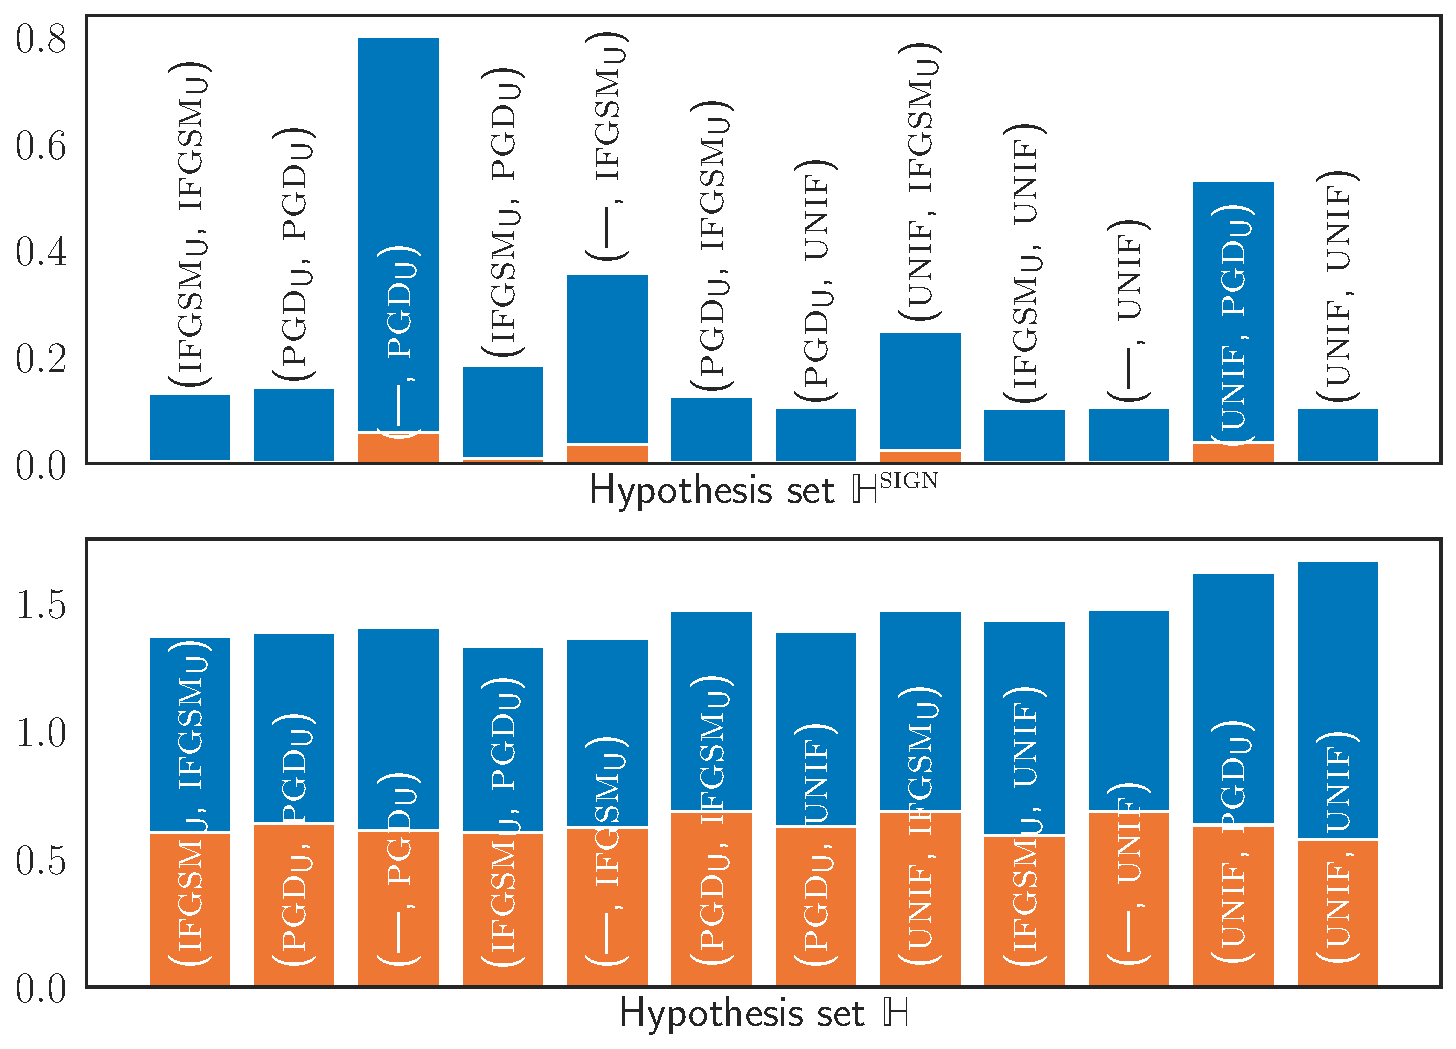
\includegraphics[width=0.8\textwidth]{chapter_3/figures/bar.pdf}
    \caption[Visualization of the impact of the TV term in \Cref{chap:mv-robustness:eq:max-mcallester}]{Visualization of the impact of the TV term in \Cref{chap:mv-robustness:eq:max-mcallester}.
    The top, respectively the bottom, bar plot show the bounds for the set of voters $\Hsigned$, respectively $\H$.
    We plot the bounds for all the scenarios of \Cref{chap:mv-robustness:tab:mnist-1-7-details} that use the $\TV$ distance, \ie, all except the pairs ($\cdot$, ---).
    In \orange{orange} we represent the value of the TV term while in \blue{blue} we represent all the remaining terms of the bound.
    }
    \label{chap:mv-robustness:fig:tv-in-bound}
\end{figure}

\paragraph{Analysis of the results.} For the sake of readability, we exhibit the detailed results for one task (MNIST:$1$vs$7$) and all the pairs (Defense,Attack) with $\ell_2$-norm in \Cref{chap:mv-robustness:tab:mnist-1-7-details}, and we report in \Cref{chap:mv-robustness:fig:tv-in-bound} the influence of the TV term in the bound of \Cref{chap:mv-robustness:theorem:bound-average-max} (\Cref{chap:mv-robustness:eq:max-mcallester}).
The detailed results on the other tasks are reported in \Cref{ap:mv-robustness:sec:additional-results}.
We provide in \Cref{chap:mv-robustness:fig:summarized-results} an overview of the results we obtained on all the tasks for the pairs (Defense,Attack) where ``$\text{Defense}{=}\text{Attack}$'' and with $\Hsigned$. 


First of all, from \Cref{chap:mv-robustness:tab:mnist-1-7-details} the bounds of \Cref{chap:mv-robustness:theorem:chromatic} are tighter than the ones of \Cref{chap:mv-robustness:theorem:bound-average-max}: this is an expected result since we showed  that the averaged-max adversarial risk $\RiskM_{\Dpert^{n\!}}(\MVQ)$ is more pessimistic than its averaged counterpart $\Risk_{\Dpert}(\MVQ)$.
Note that the bound values of \Cref{chap:mv-robustness:eq:max-mcallester-0} are tighter than the ones of \Cref{chap:mv-robustness:eq:max-mcallester}.
This is expected since \Cref{chap:mv-robustness:eq:max-mcallester-0} is a lower bound on \Cref{chap:mv-robustness:eq:max-mcallester}.

Second, the bounds with $\Hsigned$ are all informative (lower than $1$) and give insightful guarantees for our models.
For \Cref{chap:mv-robustness:theorem:bound-average-max} (\Cref{chap:mv-robustness:eq:max-mcallester}) with $\H$, while the risks are comparable to the risks obtained with $\Hsigned$, the bound values are greater than $1$, meaning that we have no more guarantee on the model learned. 
As we can observe in \Cref{chap:mv-robustness:fig:tv-in-bound}, this is due to the TV term involved in the bound. 
Considering $\Hsigned$ when optimizing $\RiskM()$ helps to control the TV term. 
Even if the bounds are non-vacuous for \Cref{chap:mv-robustness:theorem:chromatic} with $\H$, the best models with the best guarantees are obtained with $\Hsigned$.
This is confirmed by the columns $\RiskA_{\dT}(\MVQ)$ that are always worse than $\Risk_{\dTpert}(\MVQ)$ and mostly worse than $\RiskM_{\dTpert}(\MVQ)$ with $\Hsigned$.
The performance obtained with $\Hsigned$ can be explained by the fact that the sign ``saturates'' the output of the voters which makes the majority vote more robust to noises.
Thus, we focus the rest of the analysis on results obtained with $\Hsigned$.

Third, we observe that the naive defense \U is able to improve the risks $\Risk_{\dTpert}(\MVQ)$ and $\RiskM_{\dTpert}(\MVQ)$, but the improvement with the defenses based on \PGDU and \IFGSMU is much more significant specifically against a \PGDU attack (up to $13$ times better).
We observe the same phenomenon for both bounds (\Cref{chap:mv-robustness:theorem:chromatic,chap:mv-robustness:theorem:bound-average-max}).
This is an interesting fact because this behavior  confirms that we are able to learn models that are robust against the attacks tested with theoretical guarantees.

\begin{figure}
    \centering
    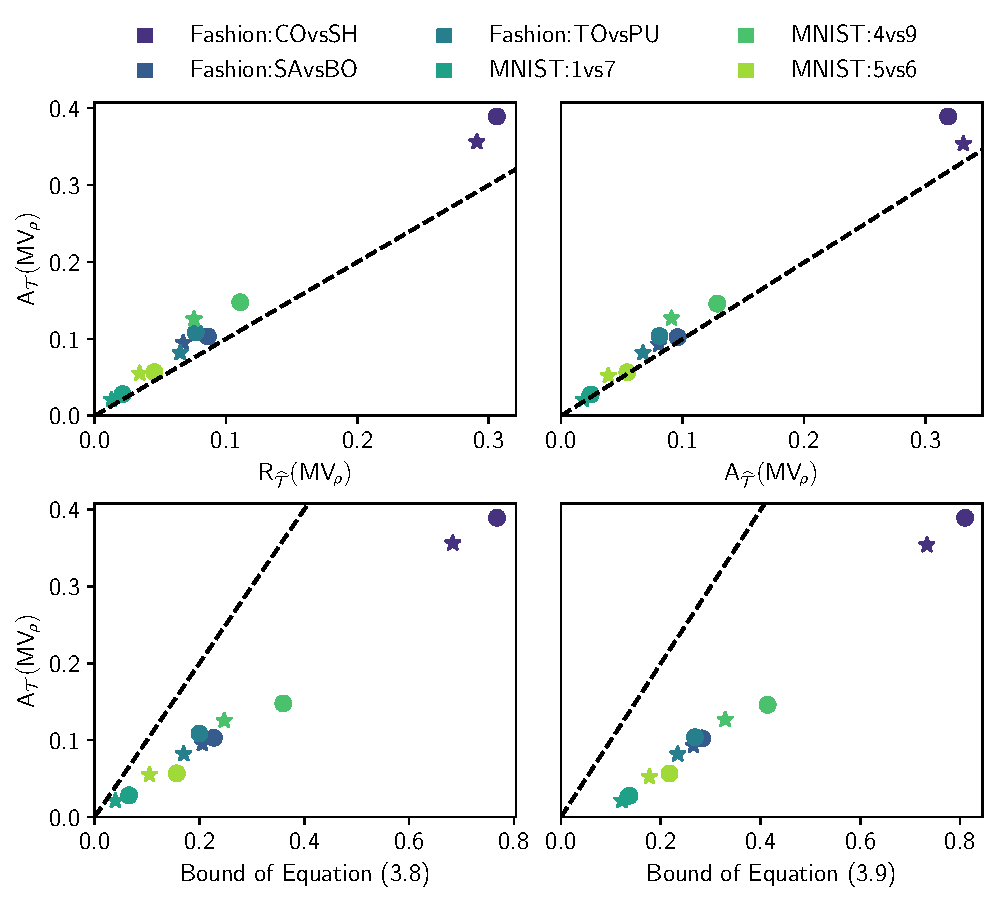
\includegraphics[width=0.8\textwidth]{chapter_3/figures/plot.pdf}
    \caption[Visualization of the risk and bound values for ``$\text{Defense}{=}\text{Attack}$'']{
    Visualization of the risk and bound values for ``$\text{Defense}{=}\text{Attack}$'' when the set of voters is $\Hsigned$.
   Results obtained with the \PGDU, respectively \IFGSMU, defense are represented by a star $\bigstar$, respectively a circle $\newmoon$ 
   {\it   (reminder: $\RiskA_{\dT}(\MVQ)$ is computed with a \PGD, respectively \IFGSM, attack).}
   The dashed line corresponds to bisecting line $y{=}x$. 
    For $\Risk_{\dTpert}(\MVQ)$ and $\RiskM_{\dTpert}(\MVQ)$, the closer the datasets are to the bisecting line, the more accurate our relaxed risk is compared to the classical adversarial risk $\RiskA_{\dT}(\MVQ)$.
    For the bounds, the closer the datasets are to the bisecting line, the tighter the bound.
   }
    \label{chap:mv-robustness:fig:summarized-results}
\end{figure}

Lastly, from \Cref{chap:mv-robustness:fig:summarized-results} and \Cref{chap:mv-robustness:tab:mnist-1-7-details}, it is important to notice that the gap between the classical risk and our relaxed risks is small, meaning that our relaxation are not too optimistic.
Despite the pessimism of the classical risk $\RiskA_{\dT}(\MVQ)$, it remains consistent with our bounds, \ie, it is lower than the bounds.
In other words, in addition to giving upper bounds for our risks $\Risk_{\dTpert}(\MVQ)$ and $\RiskM_{\dTpert}(\MVQ)$, our bounds give non-vacuous guarantees on  the classical risks $\RiskA_{\dT}(\MVQ)$.

\section{Conclusion and Summary}
\label{chap:mv-robustness:section:conclusion}

\looseness=-1
To the best of our knowledge, our work is the first one that studies adversarial robustness through the PAC-Bayesian theory for the $\Q$-weighted majority vote. 
We have started by formalizing a new adversarial robustness setting (for binary classification) with our new averaged risks.
This formulation allowed us to derive PAC-Bayesian generalization bounds on the majority vote's adversarial risk.
We illustrated the usefulness of this setting on the training of (differentiable) decision trees.
The main objective of this work was to provide some theoretical guarantees for adversarial training. 
Our aim was not to improve directly the performance of the state of the art which would require a dedicated work.\\

\looseness=-1
One of the limitation of this work is that this PAC-Bayesian analysis holds for a majority vote only.
One perspective is then to extend this work for other classifiers such as neural networks.
To do so, we can leverage the disintegrated PAC-Bayesian generalization bounds (introduced in \Cref{chap:pac-bayes:sec:disintegrated}) to bound the adversarial risk of a {\it single classifier} belonging to $\H$ and sampled from $\Q$.
Another perspective of this work is to continue analyzing the adversarial true risk of the majority vote.
Indeed, the C-Bound~\citep{LacasseLavioletteMarchandGermainUsunier2006} or the joint error~\citep{MasegosaLorenzenIgelSeldin2020} (introduced in \Cref{chap:pac-bayes:sec:surrogate}) adapted to our averaged risks might be a better choice to obtain a self-bounding algorithm since the it is more precise than twice the Gibbs risk (see \Cref{chap:pac-bayes:theorem:relationship}).
Moreover, thanks to the $\frac{1}{2}$-margin of \citet{LavioletteMorvantRalaivolaRoy2017} (recalled in \Cref{chap:pac-bayes:def:1/2-margin}), the multi-class case can be considered.\\

\looseness=-1
In the next chapters, we consider the classical supervised setting, \ie, where no inputs' perturbations are added.
For instance, \Cref{chap:mv,chap:mv-sto} focus on deriving new learning algorithms for the majority vote in the classical supervised setting.
More precisely, we derive, in \Cref{chap:mv}, the first self-bounding algorithms based on the minimization of the PAC-Bayesian C-Bound (\ie PAC-Bayesian bounds on the C-Bound).
\Cref{chap:mv-sto} presents a algorithm to minimize the risk of a PAC-Bayesian stochastic majority vote (where the distribution $\Q$ are sampled from another distribution).